\documentclass[pdf,slideColor,contemporain]{prosper}

\usepackage[latin1]{inputenc}
\usepackage{pstricks,pst-node,pst-text,pst-3d}
\usepackage{amsmath}

\newcommand{\true}{\underline{\mathrm{t}}}
\newcommand{\false}{\underline{\mathrm{f}}}
\newcommand{\undef}{\underline{\mathrm{u}}}



%%%%%%%%%%%%%%%%%%%%%%%%%%%%%%%%%%%%%%%%%%%%%%%%%%%%%%%%%%%
% slide 1
\title{\black A Real Implementation \\
        for Constructive Negation}
 \author{Susana Mu\~{n}oz ~~~~~~~ Juan Jos\'{e} Moreno}

\institution{ 
Facultad de Inform\'{a}tica  \\ 
Universidad Polit\'{e}cnica de  Madrid \\ 
28660 Madrid, Spain \\ \ \  \\
\texttt{susana@fi.upm.es} \\
\texttt{jjmoreno@fi.upm.es}  }

\begin{document}

\maketitle
%%%%%%%%%%%%%%%%%%%%%%%%%%%%%%%%%%%%%%%%%%%%%%%%%%%%%%%%%%%
\begin{slide}{Motivation}
% slide 2
\vspace{0.3cm}
     \begin{itemize}
        \item[{\blue $\bullet$}] Negation {\blue role} at Logic Programming
        \item[{\blue $\bullet$}] Problems of the {\blue proposals}:
              \begin{itemize}
                \item[$\bullet$] Complexity
                \item[$\bullet$] Expressiveness
                \item[$\bullet$] Semantics
              \end{itemize}
        \item[{\blue $\bullet$}] Limited {\blue implementations}:
              \begin{itemize}
                \item[$\bullet$] Negation as failure
                \item[$\bullet$] Delay technique
              \end{itemize}
     \end{itemize}
\end{slide}

%%%%%%%%%%%%%%%%%%%%%%%%%%%%%%%%%%%%%%%%%%%%%%%%%%%%%%%%%%%
% slide 3
\begin{slide}{Negation as failure}
\begin{itemize}

\vspace{-0.2cm}
\item[{\blue $\bullet$}] SLDNF resolution  $
         {\small
         \begin{cases}
         \begin{array}{ll}
              naf(G) :- & call(G),!, \\
                        & fail. \\
              naf(G). &
          \end{array}
          \end{cases}} $\\

\vspace{0.2cm}

\item[{\blue $\bullet$}] Execution:
\begin{tiny}
\begin{verbatim}
?- naf(even(s(s(0)))).           ?- naf(even(X)).
no                               no

?- naf(even(s(0))).              ?- naf(even(s(Y))).
yes                              no
\end{verbatim}
\end{tiny}
\vspace{0.2cm}
\item[{\blue $\bullet$}] Problem: \emph{naf} is not sound and complete.
\end{itemize}
\end{slide}

%%%%%%%%%%%%%%%%%%%%%%%%%%%%%%%%%%%%%%%%%%%%%%%%%%%%%%%%%%%
% slide 4
\begin{slide}{Interpretation of Quantif{ic}ations}

\vspace{0.5cm}
\[\mathit{\blue naf}(p(\overline{X}))~ \equiv ~ \neg \exists \overline{X}. ~ p(\overline{X})\]
\begin{itemize}

     \item[{\blue $\bullet$}] $naf(p(\overline{X})$ checks if
     $p(\overline{X})$ is ``true'' or ``false'' $\Rightarrow$
     \emph{\bf No variable instantiation}
\vspace{0.5cm}

\[\mathit{\blue cneg}(p(\overline{X}))~ \equiv ~ \exists \overline{X}. ~  \neg p(\overline{X})\]
\vspace{-0.4cm}
 
     \item[{\blue $\bullet$}]  $cneg(p(\overline{X})$ provides the values of
     $\overline{X}$ that make false $p(\overline{X})$ $\Rightarrow$
     \emph{\bf Constructive answer}
\end{itemize}
\end{slide}

%%%%%%%%%%%%%%%%%%%%%%%%%%%%%%%%%%%%%%%%%%%%%%%%%%%%%%%%%%%
% slide 5
\begin{slide}{Constructive Answers}
\vspace{-0.5cm}
\begin{small}
\hspace{-0.8cm}
\begin{verbatim}
?- cneg(even(X)).    ?- cneg(even(X)).
\end{verbatim}
{\blue \begin{verbatim}
X = s(0) ?;          X=/=0, X=/=s(s(fA(Y))) ?;
X = s(s(s(0))) ?;    X=s(s(Y)), 
                     Y=/=0, Y=/=s(s(fA(Z))) ?;
...                  ...

\end{verbatim}}


\begin{verbatim}
?- cneg(null(X)).    ?- cneg(null(X)).
\end{verbatim}
{\blue \begin{verbatim}
X = s(0) ?;          X =/= 0 ?;
X = s(s(0)) ?;       no
X = s(s(s(0))) ?;      
...                
\end{verbatim} }
\end{small}
\end{slide}

%%%%%%%%%%%%%%%%%%%%%%%%%%%%%%%%%%%%%%%%%%%%%%%%%%%%%%%%%%%
% slide 6
\begin{slide}{Constructive Negation}
     \begin{itemize}
        \item[{\blue $\bullet$}] Papers about {\blue Semantical}
        aspects

        \item[{\blue $\bullet$}] Practical {\blue Chan}'s proposal
        (coroutining)

        \item[{\blue $\bullet$}] Implementation {\blue problems}
        (Eclipse)

        \item[{\blue $\bullet$}] We provide:
              \begin{itemize}

                \item[{\blue $-$}] A complete theoretical {\blue
                algorithm} (refining and extending to the constructive
                negation method)

                \item[{\blue $-$}] A discussion about {\blue
                implementation} issues

                \item[{\blue $-$}] A preliminary implementation
              \end{itemize}
     \end{itemize}

\end{slide}

%%%%%%%%%%%%%%%%%%%%%%%%%%%%%%%%%%%%%%%%%%%%%%%%%%%%%%%%%%%
% slide 7
\begin{slide}{Negation of the Frontier}
\begin{small}
\begin{minipage}{2.5in}
{\blue
 \begin{verbatim}
even(0).
even(s(s(X))):- even(X).

 \end{verbatim}
}
\end{minipage} 
\begin{minipage}{1.5in}
{\blue
 \begin{verbatim}
 ?- cneg(even(Y)).

 \end{verbatim}
}
\end{minipage}
\end{small}

\begin{small}
$\mbox{\bf\emph{Frontier}}(even(Y)) = {\blue C_1 \vee C_2} = $ 
\[ ( Y=0 ) \vee ( \exists X~~ Y=s(s(X)) \wedge even(X) )  \] 

$\neg ~\mbox{\bf \emph{Frontier}}(even(Y)) = {\blue \neg~ C_1 \wedge
\neg~ C_2} = $ $ ~~ [ Y \neq 0 ] \wedge $\[\left[ (\forall X1.~ Y
\neq ~s(s(X1))) \vee ( (\exists X2.~ Y=s(s(X2)) \wedge \neg~ even(X2)
)\right] \]
\end{small}

\end{slide}

%%%%%%%%%%%%%%%%%%%%%%%%%%%%%%%%%%%%%%%%%%%%%%%%%%%%%%%%%%%
% slide 8
\begin{slide}{Implementation Issues}
     \begin{itemize}

        \item[$\bullet$] {\blue Disequality constraints} (Attributed
        variables) \\
        \emph{Constraints Normal Form}\\

\begin{small}

\[ \underbrace{\bigwedge_i (X_i = t_i)}_{\mbox{positive information}} \wedge~~~\] 
\[(
\underbrace{\bigwedge_j \forall~ \overline{Z}_j^1~(Y_j^1 \neq s_j^1)
\vee \ldots \vee \bigwedge_l \forall~ \overline{Z_l}^n~(Y_l^n \neq
s_l^n) )}_{\mbox{negative information}} \]


\end{small}

     \end{itemize}
\end{slide}
%%%%%%%%%%%%%%%%%%%%%%%%%%%%%%%%%%%%%%%%%%%%%%%%%%%%%%%%%%%
% slide 9
\begin{slide}{Examples}
\begin{small}

 \begin{minipage}{1.6in}
\begin{verbatim}
boole(0).
boole(1).
\end{verbatim}
\end{minipage}
\begin{minipage}{2in}
{\blue
\begin{verbatim} 
    ?- cneg(boole(X)).
    X=/=1, X=/=0 ? ;
    no
\end{verbatim} 
}
\end{minipage}\\
\vspace{0.5cm}
\begin{minipage}{1.6in}
\begin{verbatim}
positive(0). 
positive(s(X)):-
      positive(X).  
\end{verbatim}
\end{minipage}
\begin{minipage}{2in}
{\blue
\begin{verbatim} 

    ?- cneg(positive(X)).
    X=/=s(fA(_A)), X=/=0 ?;
    X = s(_A),
    _A=/=s(fA(_B)), _A=/=0 ?;
    X = s(s(_A)),
    _A=/=s(fA(_B)), _A=/=0 ? 
    yes
\end{verbatim} 
}
\end{minipage}

\end{small}

\end{slide}


%%%%%%%%%%%%%%%%%%%%%%%%%%%%%%%%%%%%%%%%%%%%%%%%%%%%%%%%%%%
% slide 10
\begin{slide}{Experimental results}
\vspace{-0.2cm}
 
\begin{tiny}

\begin{table}[t]
\begin{tabular}{||l|r|r|r|r||}
\hline %------------------------------------------------------------------
\hline %-------------------------------------------------------------------
{\bf goals} &~~ {\bf Goal} ~& ~{\bf naf(Goal) }~ &~ {\bf cneg(Goal)}~~ &~~ {\bf ratio}~~ \\ 

\hline %--------------------------------------------------------------
boole(1)                     &  2049      &  2099    &  2069   &   0.98   \\ 
\hline %--------------------------------------------------------------
positive(s(s(s(s(s(s(0))))))~~~ &  2079   &  1600    &  2159   &   1.3    \\ 
\hline %--------------------------------------------------------------
greater(s(s(s(0))),s(0))     &  2110      &  2099    &  2100   &   1.00   \\ 

\hline %-------------------------------------------------------------
\hline %-------------------------------------------------------------
{\bf average}                &            &          &         &  {\blue  1.06}   \\ 
\hline %--------------------------------------------------------------
\hline %--------------------------------------------------------------
positive(s$^{500000}$(0))             &  2930      &  2949    & 41929   &  14.21    \\ 
\hline %--------------------------------------------------------------
positive(s$^{1000000}$(0))            &  3820      &  3689    &  81840  &  22.18    \\ 
\hline %--------------------------------------------------------------
greater(s$^{500000}$(0),s$^{500000}$(0))       &  3200      &  3339    &  22370  &   7.70   \\ 
\hline %---------------------------------------------------------------
\hline %---------------------------------------------------------------
{\bf average}                &            &          &         & {\blue   14.69 } \\ 
\hline %---------------------------------------------------------------
\hline %---------------------------------------------------------------

positive(X)                  &  2020      &  -       &  7189   &          \\ 
\hline %---------------------------------------------------------------
greater(s(s(s(0))),X)        &  2099      &  -       &  6990   &          \\ 
\hline %---------------------------------------------------------------
queens(s(s(0)),Qs)           &  6939      &  -       &  9119   &          \\ 

\hline %------------------------------------------------------------
\hline %------------------------------------------------------------

\end{tabular}

\end{table}
 

\end{tiny}

\end{slide}

%%%%%%%%%%%%%%%%%%%%%%%%%%%%%%%%%%%%%%%%%%%%%%%%%%%%%%%%%%%
% slide 11
\begin{slide}{Conclusion and Future Work}
\vspace{-0.3cm}
        \begin{itemize}

                \item[{\blue $\bullet$}] Detailed description of the
                modified {\blue algorithm} (w.r.t. Chan's proposal)

                \item[{\blue $\bullet$}] Complete and consistent
                {\blue implementation}

                \item[$\bullet$] {\blue Optimizations} 

                \begin{tiny}
                \begin{itemize}
                  \item[{\blue $-$}] Compact information
                  \item[{\blue $-$}] Pruning subgoals
                  \item[{\blue $-$}] Constraint simplification
                  \item[{\blue $-$}] Finite constructive negation (cnegf)
                 \end{itemize}
                 \end{tiny}

                \item[$\bullet$] {\blue Efficiency} problem

                \begin{tiny}
                  \begin{itemize}
                  \item[{\blue $-$}] WAM level (future work)
                  \item[{\blue $-$}] Negation System for Prolog 
                  \end{itemize}
                 \end{tiny}

        \end{itemize}
\end{slide}
%%%%%%%%%%%%%%%%%%%%%%%%%%%%%%%%%%%%%%%%%%%%%%%%%%%%%%%%%%%
% slide 12
\begin{slide}{Negation System for Prolog}

  \begin{figure}
        \centering
        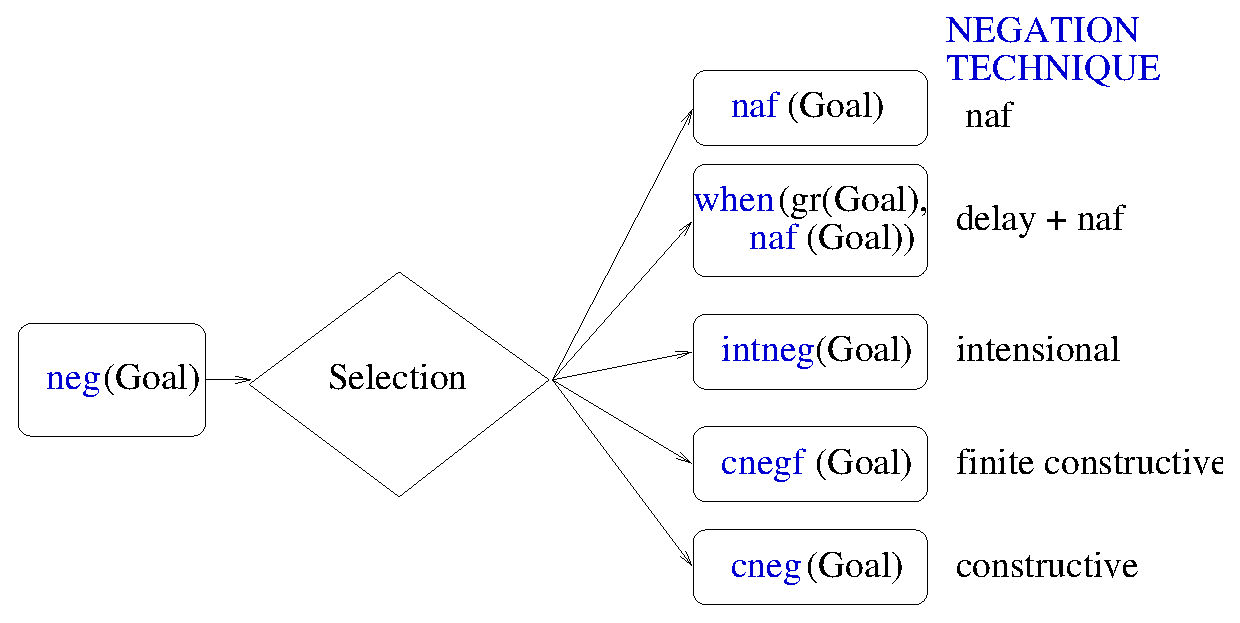
\includegraphics[width=4in]{modules.eps} 
  \end{figure}
\vspace{-0.5cm}
      \begin{itemize}
                \item[{\blue $\bullet$}] Static phase + Dynamic phase
      \end{itemize}

\end{slide}

%%%%%%%%%%%%%%%%%%%%%%%%%%%%%%%%%%%%%%%%%%%%%%%%%%%%%%%%%%%


%%%%%%%%%%%%%%%%%%%%%%%%%%%%%%%%%%%%%%%%%%%%%%%%%%%%%%%%%%%
\maketitle

\end{document} 
 
%%%%%%%%%%%%%%%%%%%%%%%%%%%%%%%%%%%%%%%%%%%%%%%%%%%%%%%%%%%


